\chapter{系统设计与实现}

本章阐述本文所设计的面向扰动水下环境新视角合成系统。本文以4D Gaussian Splatting\upcite{wu2024gaussian}为动态场景表示骨架，将SeaSplat\upcite{seasplat2025icra}中验证有效的水下物理成像模型迁移至其渲染流程；同时借鉴UDR-GS\upcite{udrgs2024symmetry}将单目深度先验融入水下动态重建的思路，由于UDR-GS未开源，本文以Depth Anything V2\upcite{yang2024depthv2}为深度先验来源对该深度监督机制进行独立实现，并将其与水下物理模块组合，形成水下物理模型、动态高斯表示与深度监督相统一的框架。本章主要工作包括：（1）给出整体管线（Pipeline）的执行流程概述；（2）将SeaSplat的后向散射、衰减子网络与水下专用损失迁移至4DGS渲染流程中，并解决两套框架在接口、参数管理和动态深度上的差异；（3）以Depth Anything V2为深度源对UDR-GS的单目深度监督思路进行独立复现，并对尺度不确定性进行处理；（4）针对多组件联合优化的不稳定性，在4DGS自身的粗精两段训练之上，进一步在精细阶段内部细分出"水下网络预热，高斯颜色调整，联合优化"的子阶段流程，这是本文针对水下动态重建提出的分阶段训练策略。

\section{总体框架设计}

\subsection{设计思路}

本文所设计的系统需要在统一框架下同时解决三个相互耦合的难题：（1）水下光学退化对颜色与对比度的干扰；（2）水流、生物游动等因素引起的动态场景变化；（3）水下场景几何重建的深度歧义性。围绕上述目标，本文采用物理解耦、动态建模与深度监督三层递进的设计思路。

\textbf{物理解耦层。}水下成像过程遵循修正的水下图像成像模型\upcite{akkaynak2018revised}，该模型将观测图像分解为干净场景辐射度与水体介质效应的叠加。本文在渲染阶段引入可学习的衰减网络（AttenuateNet）与后向散射网络（BackscatterNet）显式建模光的衰减与后向散射，使高斯点云只需学习物体本身的真实颜色，而非被水体介质叠加后的表观颜色。

\textbf{动态建模层。}4DGS通过时间条件化的变形网络（Deformation Network）对高斯点云的位置、旋转与尺度进行时序调制，并结合多分辨率特征平面（HexPlane）表达动态场景。该平面将四维时空信息分解到多个二维特征平面中，可在较低计算与存储开销下编码非刚性运动。本文继承该机制以应对水下扰动引入的非刚性运动。

\textbf{深度监督层。}水下场景往往缺乏结构光或激光测距等主动深度传感器，多视角几何约束在水体散射干扰下也易出现退化。UDR-GS\upcite{udrgs2024symmetry}已表明在4DGS框架中引入单目深度先验有助于缓解几何歧义性，本文沿用该思路；由于UDR-GS未开源，本文以Depth Anything V2\upcite{yang2024depthv2}预生成的单目逆深度图为先验，对渲染深度施加约束，引导几何收敛至合理形状，从而与水下物理建模在同一动态重建框架下协同生效。

整体处理流程为：采集多视角水下图像序列后，首先利用COLMAP进行运动恢复结构（SfM）获得稀疏点云与相机位姿；随后以稀疏点云初始化4D高斯点集，并进入本文设计的分阶段训练流程；最终系统可在任意时刻以任意视角渲染新视图。

\subsection{系统架构}

在进入各模块的具体实现之前，本节先给出整体管线的执行流程概述。在每一次训练或推理迭代中，系统首先以当前帧时刻$t$与规范空间中的高斯点集为输入，由变形网络预测各高斯基元在$t$时刻的位置、尺度与旋转偏移；随后对变形后的高斯点集执行可微分光栅化，得到干净场景颜色图$\mathbf{J}$与深度图$\mathbf{Z}$；接着，水下成像模块以$\mathbf{Z}$为输入，由后向散射网络与衰减网络分别预测后向散射图与衰减图，并结合$\mathbf{J}$按逐通道形式合成模拟观测图像$\mathbf{I}$；最后，损失函数模块在$\mathbf{I}$、$\mathbf{J}$、$\mathbf{Z}$以及单目逆深度先验之间计算重建损失、水下物理先验损失与深度一致性损失，并将梯度同时回传至高斯参数与水下网络参数。整个管线如图\ref{fig:system_architecture}所示，其中四个核心模块与上述执行流程一一对应，下面分别说明。
\begin{figure}[htbp]
  \centering
  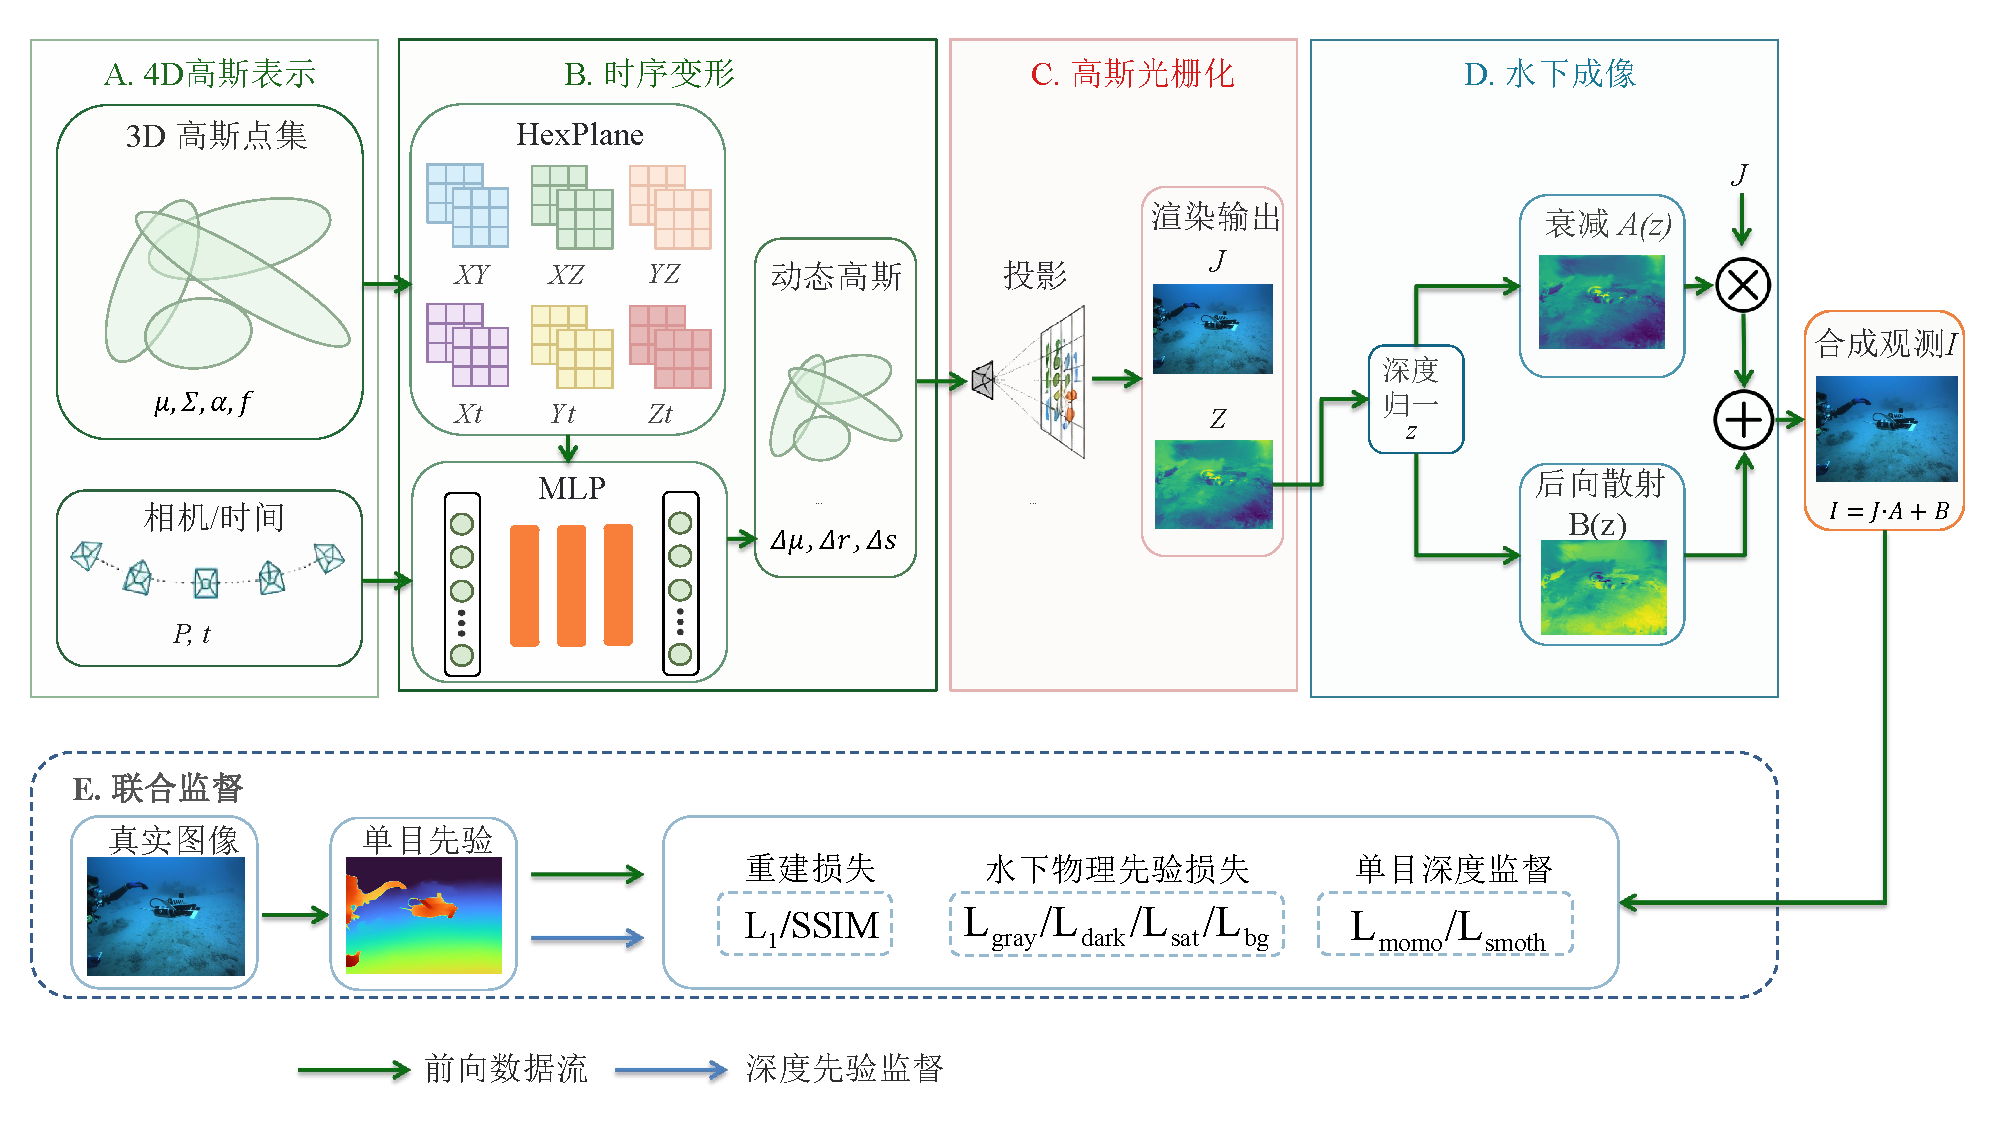
\includegraphics[width=\textwidth]{figures/pipeline.pdf}
  \caption{系统渲染管线。核心渲染流程以3D高斯点集为基础，经过变形网络调制后进行光栅化输出干净颜色图与深度图；水下成像模块基于渲染深度计算衰减与后向散射，并合成模拟观测图像；损失函数模块计算多项重建与物理先验损失，并将梯度回传至高斯参数和水下网络参数实现联合优化。}
  \label{fig:system_architecture}
\end{figure}

\textbf{（1）4D高斯点集。}场景由$N$个三维高斯椭球体参数化，每个高斯体携带位置$\boldsymbol{\mu} \in \mathbb{R}^3$、协方差$\boldsymbol{\Sigma} \in \mathbb{R}^{3\times3}$、不透明度$\alpha \in (0,1)$、球谐系数$\mathbf{f}$以及时间戳$t$\upcite{kerbl2023gaussian,wu2024gaussian}。

\textbf{（2）变形网络。}对于给定时刻$t$，多分辨率特征平面（HexPlane）与多层感知机（MLP）联合输出每个高斯体的位置增量$\Delta\boldsymbol{\mu}$、尺度增量$\Delta\mathbf{s}$和旋转增量$\Delta\mathbf{q}$，从而将规范空间中的高斯点云变形为当前帧的动态状态。

\textbf{（3）高斯光栅化。}经变形后的高斯点云通过可微分的基于分块排序的光栅化算法投影至图像平面，输出干净场景颜色图$\mathbf{J}$及深度图$\mathbf{Z}$。$\mathbf{J}$代表在无水体介质干扰时的真实辐射度。

\textbf{（4）水下成像模型。}将$\mathbf{J}$和$\mathbf{Z}$输入水下物理模型合成观测图像$\mathbf{I}$，逐通道形式为：
\begin{equation}
  I_c = J_c \cdot \exp\!\left(-\beta_c^D Z\right) + B_c^{\infty}\left(1 - \exp\!\left(-\beta_c^B Z\right)\right).
  \label{eq:uwmodel}
\end{equation}
其中，$\beta_c^D$为直接透射衰减系数，$B_c^{\infty}$为无穷远后向散射强度，$\beta_c^B$为后向散射衰减系数，均由水下网络预测。

\textbf{（5）联合优化。}将合成图像$\mathbf{I}$与真实观测图像$\mathbf{I}^{\mathrm{gt}}$进行对比，梯度同时回传至高斯参数和水下网络参数，实现联合优化。

\section{SeaSplat水下模块迁移}

\subsection{框架分析}

SeaSplat\upcite{seasplat2025icra}基于原始3DGS静态框架实现，而4DGS\upcite{wu2024gaussian}在其基础上引入了变形网络、多分辨率特征平面（HexPlane）及多分辨率哈希编码等核心组件，二者在接口设计与数据流结构上存在显著差异，迁移工作面临以下三个方面的挑战。

\textbf{渲染函数接口差异。}3DGS的渲染函数以静态高斯参数为输入，而4DGS在调用光栅化之前需先经过变形网络的时序处理，渲染函数扩展了时间戳和变形结果等额外参数。迁移时需将水下模块的介入点后移至光栅化之后，以确保输入给水下模型的颜色图$\mathbf{J}$是经过完整时序处理的干净渲染结果。

\textbf{优化器管理差异。}4DGS引入了多分辨率特征平面（HexPlane）参数和变形MLP参数两组新的可学习参数，其学习率调度策略与3DGS原有的高斯属性参数不同。本文未将水下模型参数并入原有高斯优化器，而是为后向散射网络和衰减网络分别建立独立优化器；训练时根据阶段选择执行水下优化器或高斯优化器的更新步骤，以避免两类参数的学习率调度和更新时机相互干扰。

\textbf{动态与静态表示差异。}SeaSplat假设场景静止，其推断的深度图在不同帧之间保持一致。引入4DGS后，每帧的高斯形态因变形网络而不同，导致深度图在时序上动态变化。水下物理模型必须以当前帧的实时渲染深度作为输入，而非预存的静态深度缓存。

综合考虑上述差异，迁移策略确定为在保持4DGS变形流程完全不变的前提下，在光栅化输出之后、损失计算之前插入水下成像模块实现功能集成。

\subsection{核心模块迁移}

本节给出本文从SeaSplat迁移并改写到4DGS渲染流程中的三个具体模块：后向散射网络（BackscatterNet）、直接透射衰减网络（AttenuateNet）以及四项水下专用损失函数。其中，参数初始化、独立优化器设置、阶段性更新控制以及对4DGS动态深度输入的适配均为本文针对动态框架进行的改写工作。

\textbf{后向散射网络（BackscatterNet）。}后向散射网络以归一化深度为输入，逐通道输出后向散射强度：
\begin{equation}
  B_c(Z) = \sigma(B_c^{\infty}) \cdot \left(1 - \exp(-\beta_c^B Z)\right).
  \label{eq:backscatter_impl}
\end{equation}网络结构为两层轻量卷积，参数量约1K，由独立的后向散射优化器更新。

\textbf{直接透射衰减网络（AttenuateNet）。}经消融对比，本文选用结构最简、训练更稳定的逐通道标量版本——每个通道学习一个标量衰减系数$\beta_c^D$：
\begin{equation}
  A_c(Z) = \exp\!\left(-\beta_c^D Z\right).
  \label{eq:attenuation_impl}
\end{equation}参数以较小正值初始化，使系统初始阶段接近无衰减状态，并由独立的衰减优化器更新，便于在精细阶段与后向散射网络同步完成水下物理分支的预热。

\textbf{损失函数迁移。}水下专用损失函数包含以下四个组件：

\begin{itemize}
  \item \textbf{暗通道先验损失}：基于He等人\upcite{he2011dcp}提出的暗通道先验，约束干净场景图像$\mathbf{J}$在局部窗口内至少有一个通道接近零，防止网络将水体散射残留嵌入干净图像；
  \item \textbf{灰世界先验损失}：约束干净图像每个颜色通道的均值趋向0.5，避免颜色通道间出现偏置性亮度不平衡；
  \item \textbf{RGB饱和度损失}：惩罚$\mathbf{J}$中超出$[0,1]$范围的像素值，维护物理合理性；
  \item \textbf{Alpha背景损失}：抑制相机前方水柱区域的高斯体不透明度，防止系统学习到虚假的水体填充体素，迁移过程中针对批尺寸$b=1$对掩码张量维度进行了专项修复。
\end{itemize}

\subsection{渲染流程}

在原有4DGS光栅化输出干净颜色$\mathbf{J}$和深度$\mathbf{Z}$之后，额外执行以下步骤，可参考图\ref{fig:system_architecture}的水下成像部分。

\textbf{步骤一：深度归一化。}将原始渲染深度归一化至$[0,1]$区间：
\begin{equation}
  \hat{\mathbf{Z}} = \frac{\mathbf{Z} - Z_{\min}}{Z_{\max} - Z_{\min} + \epsilon},
  \label{eq:depthnorm}
\end{equation}其中$Z_{\min}$、$Z_{\max}$为$\mathbf{Z}$的最小值与最大值。归一化可按帧动态计算或使用全局统计量；精细训练阶段采用帧级归一化以适应场景深度分布的动态变化。

\textbf{步骤二：水下网络前向传播。}将$\hat{\mathbf{Z}}$分别送入衰减与后向散射网络，按式\eqref{eq:attenuation_impl}与式\eqref{eq:backscatter_impl}逐元素得到衰减图$\mathbf{A}(\hat{\mathbf{Z}})$和后向散射图$\mathbf{B}(\hat{\mathbf{Z}})$。

\textbf{步骤三：水下成像合成。}按照式\eqref{eq:uwmodel}合成模拟水下图像$\mathbf{I}$：
\begin{equation}
  \mathbf{I} = \mathbf{J} \odot \mathbf{A}(\hat{\mathbf{Z}}) + \mathbf{B}(\hat{\mathbf{Z}}).
  \label{eq:synthesis}
\end{equation}其中$\odot$表示逐元素乘法。

上述过程整个合成路径完全可微，梯度可同时流向高斯点集参数和水下网络参数；实际参数更新则由训练阶段决定，如在水下预热阶段只更新后向散射与前向衰减参数。

\section{单目深度监督实现}

\subsection{深度图生成流程}

在水下动态重建中引入单目深度监督的思路最早由UDR-GS\upcite{udrgs2024symmetry}提出，用于缓解水下几何重建的深度歧义性。由于UDR-GS未提供开源代码，本节以Depth Anything V2\upcite{yang2024depthv2}为深度先验来源对该机制进行独立实现，并与本文迁移得到的水下物理模块及第\ref{sec:training-stages}节中的分阶段训练策略相耦合。Depth Anything V2在多种室内外场景上具备较好的跨域泛化能力，将其单目逆深度输出离线预处理后接入4DGS训练流程，能够满足实用需求。

深度图生成与处理流程如下：

（1）对数据集每张图像运行Depth Anything V2的前向推理，得到逆深度图（Inverse Depth Map）；

（2）将逆深度图归一化至$[0,255]$区间并保存为灰度图像。

选用逆深度而非线性深度的原因有以下两点：首先，水下远距离目标因散射效应造成视觉模糊，线性深度分布下远处区域的深度估计方差较大，逆深度变换可使近处高精度区域和远处区域在数值域中分布更为均匀；其次，逆深度与视差（Disparity）等价，在立体匹配和单目深度估计领域具有良好的物理解释性。

\subsection{监督机制}

\textbf{渲染深度获取。}在高斯光栅化过程中，深度图$\mathbf{Z}$通过复用颜色渲染的混合权重$w_i$对各高斯体中心深度进行加权累积得到：
\begin{equation}
  Z(\mathbf{p}) = \sum_{i} w_i(\mathbf{p}) \cdot z_i.
  \label{eq:renderdepth}
\end{equation}
其中，$\mathbf{p}$为像素坐标，$z_i$为第$i$个高斯体在相机坐标系下的深度值，$w_i(\mathbf{p})$与颜色渲染的混合权重共享，避免引入额外计算。

\textbf{尺度不确定性处理。}单目深度估计模型输出的深度图与真实度量深度之间存在未知的尺度与偏移不确定性。为消除该歧义，本文在计算损失前对渲染逆深度$d_{\mathrm{render}}$和单目逆深度$d_{\mathrm{mono}}$均进行基于均值$\mu_d$和标准差$\sigma_d$的归一化处理：
\begin{equation}
  \tilde{d} = \frac{d - \mu_d}{\sigma_d + \epsilon}.
  \label{eq:depthnorm2}
\end{equation}其中$\mu_d$表示深度图$d$在所有像素上的均值，$\sigma_d$表示对应的标准差，$\epsilon$为防止除零的小常数。此归一化操作使损失对绝对尺度不敏感，仅约束深度图的相对结构（即深度梯度与相对远近关系）与单目先验保持一致。

\textbf{损失函数。}在获得归一化逆深度后，沿用UDR-GS的整体思路，本文不直接对原始深度值施加强约束，而是将单目深度作为描述场景相对几何结构的软监督信号。具体而言，单目深度监督损失定义为归一化逆深度图之间的加权L1距离：
\begin{equation}
  \mathcal{L}_{\mathrm{mono}} =
  \frac{\sum_{\mathbf{p}} \alpha(\mathbf{p})
  \left|\tilde{d}_{\mathrm{render}}(\mathbf{p}) - \tilde{d}_{\mathrm{mono}}(\mathbf{p})\right|}
  {\sum_{\mathbf{p}} \alpha(\mathbf{p}) + \epsilon}.
  \label{eq:depthloss}
\end{equation}其中，$\alpha(\mathbf{p}) \in [0,1]$为像素$\mathbf{p}$处的高斯累积透明度，对高斯覆盖良好的区域给予更高监督权重，对空白背景区域减少干扰；分母中的$\sum_{\mathbf{p}}\alpha(\mathbf{p})+\epsilon$用于对有效监督区域进行归一化，使不同视角、不同前景覆盖面积下的损失幅值保持相对稳定。采用逆深度形式的原因在于，近景区域对新视角合成中的遮挡关系和局部几何误差更为敏感，逆深度能够在数值上增强近处结构的约束；同时，均值方差归一化消除了Depth Anything V2预测结果中的全局尺度和偏移不确定性，使该损失主要关注物体轮廓、深度层次和相对远近关系，而不强制渲染深度与单目估计在绝对尺度上一致。该损失与光度重建损失共同作用：光度项约束图像颜色一致性，单目深度项则抑制水下散射、低纹理区域和动态扰动造成的高斯漂浮与局部深度塌缩，从而提升高斯场景表示的几何稳定性。

\textbf{配置参数。}实现中需要指定单目深度先验的存放目录，并声明预存文件为逆深度格式，同时启用单目深度监督开关。深度监督损失权重$\lambda_{\mathrm{mono}}$设定为0.1，并配合热启动调度策略在训练初期逐步引入。

\section{分阶段训练策略}
\label{sec:training-stages}

分阶段训练策略用于降低多组件联合优化的不稳定性。当水下网络、变形网络与高斯点集同时从零开始优化时，颜色退化、几何误差和动态形变误差会在同一光度损失中相互干扰：水下网络若过早引入，可能把几何错位解释为后向散射或衰减；变形网络若在几何尚未稳定时充分更新，则容易把水体造成的颜色差异误当作运动信号。为此，本文不直接启动全部模块，而是先优化几何结构，再使用独立优化器预热水下分支，最后交替控制高斯参数与后向散射与前向衰减参数的更新。

本文的训练流程继承了4DGS\upcite{wu2024gaussian}原有的两阶段框架：粗训练阶段在不开启水下物理模型的条件下与原始4DGS等价，用于建立基础几何结构；精细训练阶段则启用水下模块、深度监督等本文新增的组件。本文的工作集中于精细训练阶段，针对水下网络、动态高斯属性与深度监督之间的梯度耦合，将其进一步细分为"后向散射与前向衰减参数预热—高斯颜色调整—联合训练"三个子阶段，并在联合训练阶段交替更新高斯参数和水下模块。实现中通过跳过高斯优化器步骤，使预热和间歇式专项更新只作用于后向散射网络与衰减网络。完整的阶段划分及各阶段中的可学习参数与损失项配置如图\ref{fig:training_stages}所示。

阶段划分对应三类优化对象的启停边界：高斯几何与密度控制首先建立可渲染的基础结构；水下参数随后在固定几何上估计衰减和后向散射的量级；高斯颜色再在相对稳定的水下参数下校准到干净外观空间；最后进入联合训练，交替更新高斯参数和水下模块。该策略本质上是训练稳定性设计。

\begin{figure}[htbp]
  \centering
  \begin{tikzpicture}[
  font=\footnotesize,
  >=Stealth,
  stage/.style={
    draw=#1!75!black,
    fill=#1!12,
    rounded corners=2pt,
    line width=0.7pt,
    minimum height=1.0cm,
    text width=2.6cm,
    align=center,
    inner sep=4pt
  },
  stage/.default=orange,
  group/.style={
    draw=#1!70!black,
    dashed,
    rounded corners=4pt,
    line width=0.6pt,
    inner sep=8pt
  },
  note/.style={font=\scriptsize, align=center, text=black!75},
  arr/.style={->, line width=0.75pt, draw=black!70}
]

% ===== Stage row =====
\node[stage=cyan]   (s1)                       {粗训练阶段\\\scriptsize iter 0--3000};
\node[stage=orange, right=0.6cm of s1] (s2)    {BS/AT 预热\\\scriptsize iter 3000--4000};
\node[stage=red,    right=0.6cm of s2] (s3)    {高斯颜色调整\\\scriptsize iter 4000--6000};
\node[stage=purple, right=0.6cm of s3] (s4)    {联合训练\\\scriptsize iter 6000--20000};

\draw[arr] (s1) -- (s2);
\draw[arr] (s2) -- (s3);
\draw[arr] (s3) -- (s4);

% ===== Key annotation under each stage =====
\node[note, below=0.15cm of s1] {更新高斯几何与颜色\\水下模块未启用};
\node[note, below=0.15cm of s2] {更新BS/AT\\冻结高斯几何与颜色};
\node[note, below=0.15cm of s3] {仅更新高斯颜色\\冻结高斯几何与BS/AT};
\node[note, below=0.15cm of s4] {全参数联合更新\\并间歇式专项更新 BS/AT };

% ===== Group framing =====
\begin{scope}[on background layer]
  \node[group=cyan, fit=(s1)] (g1) {};
  \node[group=orange, fit=(s2)(s3)(s4)] (g2) {};
\end{scope}

\node[note, text=cyan!55!black, above=0.05cm of g1.north]   {粗阶段};
\node[note, text=orange!55!black, above=0.05cm of g2.north] {精细阶段子流程};

\end{tikzpicture}

  \caption{分阶段训练策略流程图。最外层的粗训练与精细训练两段框架继承自4DGS（蓝色虚线框），本文在精细训练阶段内部进一步细分出后向散射与前向衰减参数预热、高斯颜色调整与联合训练三个子阶段（橙色虚线框），并在联合训练阶段引入间歇式专项更新。}
  \label{fig:training_stages}
\end{figure}

\subsection{粗训练阶段}

该阶段位于训练流程的起始部分，在水下物理模型尚未激活的条件下，系统等价于原始 4DGS 训练，用于建立场景的基础几何骨架。损失函数为：
\begin{equation}
  \mathcal{L}_{\mathrm{coarse}} = (1-\lambda_{\mathrm{s}})\mathcal{L}_1(\mathbf{J}, \mathbf{I}^{\mathrm{gt}}) + \lambda_{\mathrm{s}} \mathcal{L}_{\mathrm{D}\mbox{-}\mathrm{SSIM}}(\mathbf{J}, \mathbf{I}^{\mathrm{gt}}).
  \label{eq:losscoarse}
\end{equation}
其中，$\lambda_{\mathrm{s}}=0.2$为结构损失权重，$\mathcal{L}_{\mathrm{D}\mbox{-}\mathrm{SSIM}}$表示由SSIM构造的结构差异项。此阶段开启自适应密度控制（Adaptive Density Control），执行高斯体的分裂、克隆与修剪操作，建立场景的基础几何骨架。为避免视角相关颜色效应与后续水下模型产生干扰，球谐阶数固定为0，使每个高斯体只学习与视角无关的漫反射颜色。

\subsection{精细阶段初始化}

在粗训练完成之时，系统执行一次性的精细阶段初始化，该阶段在图\ref{fig:training_stages}未显示：创建并启用后向散射网络与衰减网络，并分别为二者建立优化器。选用粗训练阶段学习到的背景颜色对后向散射网络的$B^{\infty}$参数进行初始化，使其从一个合理的先验值起步，加速精细阶段的收敛。

在初始化完成的第一个迭代步内，高斯体的位置、不透明度、缩放、旋转和颜色参数被临时冻结，防止刚启用水下模型时不稳定的梯度影响几何结构；下一迭代步起即解冻后向散射与前向衰减参数进入预热阶段。

\subsection{后向散射与前向衰减参数预热阶段}

该阶段冻结高斯点集所有参数，仅执行后向散射与前向衰减参数的更新，在高斯几何不受干扰的条件下，让水下物理模型快速捕捉水体介质的光学特性（各通道衰减系数的量级与后向散射基准强度），为后续联合优化提供稳定的水下模型初始化。此时损失仍由图像重建项和水下相关约束共同决定，但高斯优化器不执行更新。

\subsection{高斯颜色调整阶段}

水下物理模型预热完成后，切换至高斯颜色调整阶段，暂停后向散射与前向衰减参数更新，转而执行高斯颜色参数更新，用于校准高斯点集的颜色属性。其目的在于，在水下网络基本确定水体介质参数的前提下，让高斯颜色在去水体后的干净颜色空间中重新校准，使$\mathbf{J}$逐步逼近真实物体的本征颜色，而非被水体污染的表观颜色。

\subsection{联合训练阶段}

在高斯颜色完成初步对齐后，训练进入末段的联合训练阶段：高斯点集与水下物理模型的参数交替更新：

\begin{itemize}
  \item 在每个完整更新周期内，按预设比例插入若干步的水下物理模型专项更新，此时只执行后向散射与衰减参数的更新步骤，并跳过高斯参数更新；
  \item 其余迭代步执行高斯优化器步骤，并跳过水下参数更新，使动态高斯表示继续根据重建损失和深度监督进行调整。
\end{itemize}

该机制的物理动机是，随着场景几何的持续改变（高斯点云的位置和密度在联合优化中仍会变化），渲染深度图$\mathbf{Z}$也随之改变，需要定期给水下网络提供独立的优化机会，使其适应几何变化。

完整损失函数在该阶段激活全部组件：
\begin{equation}
  \begin{aligned}
    \mathcal{L} =\ & \mathcal{L}_1 + \lambda_{\mathrm{s}}\mathcal{L}_{\mathrm{D}\mbox{-}\mathrm{SSIM}}
                  + \lambda_{\mathrm{smooth}}\mathcal{L}_{\mathrm{smooth}}
                  + \lambda_{\mathrm{dark}}\mathcal{L}_{\mathrm{dark}} \\
                & + \lambda_{\mathrm{gray}}\mathcal{L}_{\mathrm{gray}}
                  + \lambda_{\mathrm{sat}}\mathcal{L}_{\mathrm{sat}}
                  + \lambda_{\mathrm{bg}}\mathcal{L}_{\mathrm{bg}}
                  + \lambda_{\mathrm{mono}}\mathcal{L}_{\mathrm{mono}}.
  \end{aligned}
  \label{eq:lossfull}
\end{equation}
各损失项含义如下：$\mathcal{L}_1$为像素级L1重建损失；$\mathcal{L}_{\mathrm{D}\mbox{-}\mathrm{SSIM}}$为由结构相似性指数\upcite{wang2004ssim}构造的结构差异损失；$\mathcal{L}_{\mathrm{smooth}}$为深度平滑正则项，约束渲染深度图在空间上的平滑性；$\mathcal{L}_{\mathrm{dark}}$为暗通道先验损失\upcite{he2011dcp}；$\mathcal{L}_{\mathrm{gray}}$为灰世界先验损失；$\mathcal{L}_{\mathrm{sat}}$为RGB饱和度损失；$\mathcal{L}_{\mathrm{bg}}$为Alpha背景损失；$\mathcal{L}_{\mathrm{mono}}$为单目深度监督损失（式\eqref{eq:depthloss}）。

为防止训练初期损失震荡，各辅助损失项采用线性热启动（Warm-Up）调度策略：
\begin{equation}
  w(k) = w_{\mathrm{base}} \cdot \max\!\left(0,\; \min\!\left(1,\; \frac{k - k_{\mathrm{start}}}{k_{\mathrm{ramp}}}\right)\right).
  \label{eq:warmup}
\end{equation}
其中，$k$为当前迭代步，$k_{\mathrm{start}}$为该损失项的激活步，$k_{\mathrm{ramp}}$为热启动步数（默认500步）。

\section{本章小结}

本章详细介绍了面向扰动水下环境的新视角合成系统的完整设计与实现。主要内容包括：（1）以4DGS为骨架、SeaSplat水下物理模型为外层包装、Depth Anything V2为深度先验的三层系统架构设计；（2）SeaSplat核心水下模块（后向散射网络、衰减网络及多项水下专用损失）向4DGS框架的迁移方案；（3）借鉴UDR-GS将单目深度先验融入水下动态重建的思路，由于UDR-GS未开源，本文以Depth Anything V2为深度源对该机制进行了独立实现并处理了尺度不确定性；（4）在4DGS自身粗-精二段框架之上，针对精细阶段内部多组件梯度干扰所设计的子阶段训练策略。
